%http://mathematica.stackexchange.com/questions/11350/xkcd-style-graphs
\documentclass[12pt]{article}
\usepackage[authoryear]{natbib}
\usepackage[margin=1.0in]{geometry}
\usepackage{pseudocode}
\usepackage{mathtools}
\usepackage{datetime}\usepackage{hyperref}
\usepackage{amsmath}
\usepackage{amsfonts}
\usepackage{graphicx}
\usepackage{bookman}
\usepackage{pgfplotstable}%for generating latex from csv files
\usepackage{booktabs}
\usepackage{cmbright}

%\usepackage{ccfonts,eulervm}
%\usepackage[T1]{fontenc}

% \usepackage{ccfonts}
% \usepackage[T1]{fontenc}

\title{``A New Series Representation for Time Invariant Functions and
a Solution Strategy for Occasionally Binding Constraints in Rational Expectations Models''}
\date{\currenttime -- \today }



\author{Gary S. Anderson\thanks{I would like to thank Luca Guerrieri, Christopher Gust and Robert Tetlow for their comments and suggestions. }}
\newcommand{\xtFuncTI}{\mathcal{X}(x,\epsilon)}
\newcommand{\XtFuncTI}{\mathbf{X}(x)}

\newcommand{\xtFunc}[1]{\mathcal{X}{#1}}
\newcommand{\XtFunc}[1]{\mathbf{X}{#1}}



\newcommand{\discr}[1]{\mathcal{D}^{#1}(x_{t-1},\epsilon_t)}

\newcommand{\XZPair}[1]{(\mathcal{X}^{#1},\mathcal{Z}^{#1})}
\newcommand{\XZPairG}[1]{(\mathcal{X}^{#1}(x^g),\mathcal{Z}^{#1}(x^g))}
\newcommand{\xIter}[2]{\mathcal{X}^{#1}(#2)}
%\newcommand{\zNow}[1]{z^{#1}_0(x_{t-1},\epsilon_t)}
%\newcommand{\ZNow}[3]{\mathcal{Z}^{#1}_{#2}(x_{#3})}
\newcommand{\zNow}[1]{z^{#1}(x_{t-1},\epsilon_t)}
\newcommand{\ZNow}[3]{\mathcal{Z}^{#1}(x_{#3})}

\newcommand{\xNow}[1]{x^{#1}_t(x_{t-1},\epsilon_t)}
\newcommand{\xNowtp}[1]{x^{#1}_{t+1}(x_{t-1},\epsilon_t)}
\newcommand{\XNow}[3]{\mathcal{X}^{#1}_{#2}(x_{#3})}








\newcommand{\sForSum}{{\nu}}
\newcommand{\rcpC}{{\mathbf{c}}}

\newcommand{\xtVec}{  \begin{bmatrix}
    q_t\\r_{t}\\r_{ut}
  \end{bmatrix}
}
\newcommand{\xtPVec}{  \begin{bmatrix}
    q_{t+1}\\r_{t+1}\\r_{ut+1}
  \end{bmatrix}
}
\newcommand{\xtMVec}{  \begin{bmatrix}
    q_{t-1}\\r_{t-1}\\r_{ut-1}
  \end{bmatrix}
}
\newcommand{\expctEps}[1]{\mathcal{E}_{\epsilon} \left [#1 \right ]}
\newcommand{\expct}[2]{E_{#1} \left [#2 \right ]}
\newcommand{\expc}[1]{\mathcal{E} \left [#1 \right ]}
\newcommand{\expcK}[2]{\mathcal{E}^{#1} \left [#2 \right ]}
\newcommand{\xsln}[1]{\mathbb{X} \left [#1 \right ]}
\newcommand{\xslnK}[2]{\hat{\mathbb{X}}^{#1} \left [#2 \right ]}
\newcommand{\xpth}[2]{\mathfrak{X}_{#1} \left [#2 \right ]}
\newcommand\infNorm[1]{\left\lVert#1\right\rVert_\infty}
\newcommand\twoNorm[1]{\left\lVert#1\right\rVert_2}
%\newcommand{\inorm}[1]{\left\lVert#1\right\rVert_\infty}

% \newcommand{\forPhi}{\begin{bmatrix}
% \psi_\epsilon&\psi_z
% \end{bmatrix}}
% \newcommand{\phiMult}{\phi \psi_\epsilon}
% \newcommand{\bMult}{B x_{-1} + \phiMult}
\newcommand{\phiMultBoth}[1]{
	\phi (\psi_\epsilon \epsilon_t +\psi_z z_0^#1(x_{-1},\epsilon_t))}
\newcommand{\bMultBoth}[1]{B x_{-1} + \phiMultBoth{#1}}


\newcommand{\bForOne}{\bMultBoth{1}
}

% \newcommand{\bForTwo}{\bMultBoth{2}+
% F \phi  \psi_z  
% Z_0^1(x_0^2(x_{-1}))   
% }



\newcommand{\compSlack}{z_0^1(x_{-1},\epsilon_t) \left ( \bar{x} -x\right )=0\\ z_0^1(x_{-1},\epsilon_t)> 0}
% \begin{gather*}
% 0= x_t-(B x_{t-1}+ \phi \psi_\epsilon\epsilon_t + \phi \psi_z 
% \xpt{z_{t}(x_{t-1},\epsilon_t)    } )
% \end{gather*}

\newcommand{\xpt}[1]{#1}


\makeatletter
\@ifundefined{newblock}{%
 \def\newblock{\hskip .11em plus .33em minus .07em} % important line
}
\makeatother


\makeatletter
\pgfplotsset{
    /pgfplots/table/omit header/.style={%
        /pgfplots/table/typeset cell/.append code={%
            \ifnum\c@pgfplotstable@rowindex=-1
                \pgfkeyslet{/pgfplots/table/@cell content}\pgfutil@empty%
            \fi
        }
    }
}
\makeatother
 

\makeatletter
\newcommand*\ExpandableInput[1]{\@@input#1 }
\makeatother


\newcommand{\tpExp}[1]{\phi^e_{#1}(x_{t-1})}
\newcommand{\lRat}[2]{\log \left( \frac{z_{#1}}{z_{#2}}\right)}


\newcommand{\anEdit}[1]
{

{\color{blue}
\begin{quote}
#1  
\end{quote}}

}

\mathtoolsset{showonlyrefs}

\pgfplotstableset{fixed zerofill,precision=8}
\begin{document}
\maketitle

\begin{abstract}


 
This paper proposes a new representation for time invariant functions.
This series representation 
can accurately characterize the solutions for a 
wide array of nonlinear rational expectations models 
and provides a formula
for computing accuracy bounds for any proposed time invariant model solution.
The series representation serves as an important component in an algorithm 
for constructing approximate solutions for nonlinear rational expectations
models.
In this context, it  facilitates exploiting the 
``law of iterated expectations'' in computing rational expectations solutions for models with occasionally binding constraints.


\end{abstract}

 \newpage
 \tableofcontents
 \newpage


\section{Introduction and Summary}

Economists are increasingly interested in building and solving 
economic models that honor/include occasionally binding constraints.
Since \cite{Christiano2000} authors have described a 
variety of approaches.\cite{holden15:_exist_dsge,guerrieri15:_occbin,benigno09,hintermaier10,brumm10,nakov08,haefke98,nakata12,gordon11,billi11,Hintermaier2010,Guerrieri2015}
These approaches typically specify a solution that characterizes a family of
time invariant functions.

Since these models cannot be solved exactly, each approach requires an
approximation method and an iteration with a stopping criterion.
It is problematic to decide when the solution is good enough.

The text describes a methodology for computing an error bound on the 
size of the change that one can expect from modifying the trajectory of the 
solutions.

\begin{itemize}
\item To solve a wide class of useful but increasingly complex models. 
\item Time invariant functions ubiquitous in economic models
\item Approximation error for time invariant functions help us choose how to allocate resources during calculations
\item Occasionally binding constraints increasingly a part of economic models
\item Impulse Response functions and Potter connection to conditional expectations
\item Source of decision rule irrelevant --  Perturbation, projection, as long as time invariant criterion can assess impact of discrepancies.
\item leads naturally to the specification of a robust algorithm
\end{itemize}



Judge using impulse response functions.\cite{Potter2000}
\section{Methodology Outline}

\subsection{Model Context}
\label{sec:model-context}

This section will suggest that the range of applicability is wide but
hard to characterize.
Should be useful anyplace that bounded time invariant functions appear.

We focus on models with time invariant decision rule solutions. 
It is difficult to characterize the model specification, but easier to specify the common characteristics of the solutions.  A s a consequence the approach is very general the text will provide a variety of models that would be amenable, but the list is not meant to be exhaustive.


The proofs of applicability 
turn on being able to rely on the law of iterated expectations and time invariant functions.
It is difficult to think of economic models  that don't exploit these features.
We require models that have solutions, decision rules, that produce unique paths when iterated forward.  

What is meant my iterating a decision rule depends upon assumption about the
model and the stochastic component if any.
We will  touch on two widely used approaches: Rational expectations and 
perfect foresight. The theory and the algorithms would apply for any method which obeys the law of iterated Expectations.

\subsection{General Methodology}
\label{sec:general-methodology}



Consider any bounded deterministic family of functions 
\begin{gather}
  \mathcal{X}_{t+s}(x_{t-1},\epsilon_t), \,\,\mathcal{X}_{t+s} \in{R^k}\,\,\infNorm{\mathcal{X}_{t+s}}  \le \bar{\mathcal{X}}\,\,\forall s\ge 0 \label{fFamily}.
\end{gather}
Where $\epsilon_t$ is the realization of an r dimensional iid random shock  known at time t. The $x_{t-1}$ are endogenous state variables fixed by history.  
In what follows, these functions will represent the time t conditional expectations of solutions for dynamic stochastic models which may be subject to occasionally binding constraints.  These functions are indexed by the variables $x_{t-1}, \epsilon_t$ so that each member of the family characterizes the evolution of a deterministic trajectory of values.

From what to what.  $\forall t (-\infty,\infty)$ 

Consider a time invariant function $\xtFuncTI$, where $x$ is an $L$ dimensional real variable and $\epsilon$ a $K$ dimensional random variable. 
We will require
the time $t$ realizations of $\epsilon$, $\epsilon_t$, to be independently and identically distributed.
We define a time invariant function $\XtFuncTI\equiv \expctEps{\xtFuncTI}$ and denote
\begin{gather*}
\expct{t}{x_{t+k}}\equiv\begin{cases}
\xtFunc{(x_{t-1},\epsilon_t)} &k=0\\
\XtFunc{(\expct{t}{x_{t+k-1}})} &k>0
\end{cases}
\end{gather*}
The function $\expctEps{\cdot}$ may be a mathematical expectation, for rational expectations, or a function which assigns the value $0$ to all future $\epsilon_t$ for perfect foresight solutions.
In the text that follows, we will assume that at time $t$, $\epsilon_t$ along with all the history $x_{t-k},\, \forall k>0$ are known.
Note that as a result, 
$\xtFunc{(x_{t-1},\epsilon)}$ and 
$\expct{t}{x_{t+k}}$ are deterministic functions.  

This will facilitate the solution of difficult decision problems such as problems with
occasionally binding constraints. Many of the calculations we will do exploit the ``Law of Iterated Expectations,'' so we make its validity explicit now.


With these conventions,  it is possible with invariant functions to iterate the solutions forward.
If these solutions remain bounded, we will see that there is a useful series representation
 reproducing these trajectories.\footnote{The algorithm turns on using the law of iterated expectations property.
Consequently, it will also work for degenerate distributions.  Since the first
period is deterministic,  perfect-foresight solutions 
where all future shocks are zero fit the formula.
}



  \subsection{A  Series Representation for Time Invariant Functions}


Now, for any linear homogeneous 
$k$ dimensional 
deterministic 
system, 
\begin{gather}
  	 H_{-1} x_{t-1} + H_0 x_t + H_1 x_{t+1}=0\label{hSystem}
\end{gather}
that produces  a unique stable solution, 
it is well known\ \cite{anderson10} that
one can write the solution for corresponding inhomogeneous stochastic models\footnote{Any variable that can be influenced by the time $t$ stochastic shock must be dated $t$ or later.}\footnote{I conjecture that the eigenvalues of F will correspond to the reciprocal of the large eigenvalues in the model and are consequently strictly less than 1 in the models we will address.  For bounded 
 $Z$ functions, the series will converge. It will also then be the case that $(I-F)^{-1}$ exists.}
\begin{gather}
	 H_{-1} x_{t-1} + H_0 x_t + H_1 x_{t+1}=\psi_\epsilon \epsilon_t +\psi_{c}
\intertext{as}
x_t=B x_{t-1} + \phi \psi_\epsilon \epsilon_t + (I - F)^{-1} \phi \psi_c
\intertext{where}
\phi= (H_0 +H_1 B)^{-1} %\\F=-\phi H_1 
\end{gather}

Given the trajectories \refeq{fFamily}, define 
$  z_{t+s}(x_{t-1},\epsilon_t)$ as  \footnote{These $z$ functions will soon prove useful in an algorithm for computing 
unknown trajectories like \refeq{fFamily}.
}:
{

  \begin{align}
  z_{t+s}(x_{t+s-1},\epsilon_t) \equiv& H_{-1} \mathcal{X}_{t-1}(x_{t+s-1},\epsilon_t) + \nonumber\\
& H_0 \mathcal{X}_{t+s}(x_{t-1},\epsilon_t) +  \label{defZ} \\
& H_1 \mathcal{X}_{t+s+1}(x_{t-1},\epsilon_t) \nonumber
  \end{align}
}


\cite{anderson10}  demonstrates that, for 
such models,
	 \begin{gather}
	 \mathcal{X}_{t}(x_{t-1},\epsilon_t) =B x_{t-1}+ \phi \psi_\epsilon\epsilon_t + \sum_{\sForSum=0}^\infty F^s \phi z_{t+\sForSum}(x_{t-1},\epsilon_t) + (I - F)^{-1} \phi \psi_c
\label{theSeries}\intertext{and}
	 \mathcal{X}_{t+s+1}(x_{t-1},\epsilon_t) =B \mathcal{X}_{t+s} + \sum_{\sForSum =0}^\infty F^\sForSum \phi z_{t+s+\sForSum}(x_{t-1},\epsilon_t) + (I - F)^{-1} \phi \psi_c \,\,\,\forall s \ge  0\nonumber
\intertext{where}
F=-\phi H_1 
	 \end{gather}
	 Consequently, given a family of trajectories like those in \refeq{fFamily},
and a stable linear homogeneous system like \refeq{hSystem},
one can easily compute a series 
representation for a function generating the family of
trajectories.
Interestingly, the formula will work for any 
$k$ dimensional linear system with unique  stable solutions.
Consequently, the linear model and the  constant term can  be chosen rather
 arbitrarily.  This observation will give us some confidence in the 
robustness of our algorithm of section \ref{sec:unknown-solutions} for constructing series 
representations for unknown families of functions 
satisfying a given system of equations over time.

One could consider approximating $x_t(x_{t-1},\epsilon_t)$ by 
truncating the series at a finite number of terms.
 	 \begin{gather}
 	 x_{t}(x_{t-1},\epsilon_t,k) \equiv B x_{t-1}+ \phi \psi_\epsilon\epsilon_t + \sum_{s=0}^k F^s \phi z_{t+s}(x_{t-1},\epsilon_t)  \label{theTruncSeries}\\ %+ (I - F)^{-1} \phi \psi_c
\intertext{
 As shown in appendix \refeq{truncForm}, one can bound the error in the 
approximation of $x_t$.
}
 	\infNorm{x_{t}(x_{t-1},\epsilon_t) -x_{t}(x_{t-1},\epsilon_t,k)} \le 
  \infNorm{ (I -F)^{-1} F^{k+1}\phi} \bar{\mathcal{X}}
 \end{gather}
Since the eigenvalues of F are all less than one, one can expect the approximation to improve as terms are added.


Given a time invariant function that generates a family of bounded solutions for a range of initial conditions we have a method for constructing a time series
replicating those trajectories.  
Many well known economic models generate solutions consisting of
a family of invariant functions.
Typically, these solutions cannot be computed in closed form and consequently
obtained by some numerical method.
Below, we will describe a method for constructing the time invariant solutions
for a given model, but 
it will be useful to begin by considering a model with know solutions.
We will see how to characterize the accuracy of a given representation of the time invariant function.  In the context of a model that generates
solutions that are time invariant and bounded, we can use the 
series representation to  assess the accuracy of a proposed solution.

Along the path, check if conditional expectations correct.  If not use the conditional expectation in addition to the hmat to measure the error.

We can assess, at least locally, 
how well a particular proposed solution performs.

\subsection{Assessing a Proposed Solution}
\label{sec:decis-rule-assessm}

Must use ``chunks'' to augment the system in such a way that we
can use the ``law of iterated expectations''.
Everywhere that a collection of 
$t+1$ variable appears together, non linearly they must be subsumed in an
auxiliary variable, a ``chunk'', 
that will be defined at time $t$.  As a result, at each step
of the iteration that arises, the time $t$
conditional expectation of that chuck will appear in the 
linear reference model and can be accurately computed and
used in subsequent calculations.


Iteration:
\begin{gather}
\underbrace{(x_{t-1},\epsilon_t)} 
\underbrace{DR(x_{t-1},\epsilon_t)}
\underbrace{\int DR(DR(x_{t-1},\epsilon_t),\epsilon_{t+1}),\epsilon_{t+1})}
\underbrace{\ldots}
\end{gather}

Evaluating equation system along path shows solutions valid. Discrepancies call for a path change.

\label{sec:assess}
\begin{itemize}
\item Iterate the decision rule forward.  The rule should compute a path for conditional expectations from an arbitrary set of initial conditions.
\item compute errors along the path
\item employ the formula to compute the amount that the initial value should change
\item could update this path with those values for perfect foresight
just need for a single point zero error done for rational expectations 
i think multiple path updates necessary could be done in parallel perhaps at each of the interpolation points of the Z approximation
\item use truncation formula to bound impact
\end{itemize}









\begin{itemize}
\item simulate paths for conditional expectations
\item evaluate model along the path
\item use errors and formula to improve path 
\item repeat and correct
\item conditional expectations
\item model errors
\item bounds
\item how can multiplicities matter?  
\item how can terminal constraints matter?
\item bimodal distributions for dist of Z
\end{itemize}



We typically have a model we are interested in and would like to compute an approximate solution.  For now assume that the model imposes a time invariant system of equations on the model variables.
The source of the decision rule doesn't matter.  So long as we can iterate the
rule forward in time to produce a family of bounded paths, we can use the
formula to assess how close the solutions are to solving the particular.
We need only compute the paths, apply the model equations to the path to determine how much the system equations are violated.  These calculations will 
generate a path for the $z$ functions.  Substituting these values in the
formula provides a measure of how much the $x_t$ must change in order for the conditional expectations path to satisfy the model equations.
The model equations can be highly complex. Some of the examples hint at the 
possibilities. Occasionally binding constraints addressed in a straightforward 
way.  Conceptually, the approach is compelling.  The examples below
offer some practical numerical insights in early implementation of these
ideas.



We will need to ``simulate'' the decision rule forward in order to judge if the conditional expectations are correct.
We can try iterating the perfect foresight solution forward to see how well the formula predict the discrepancy.  Can vary the variance to see that it's okay for small variance.

We will need to choose a horizon length. We can simulate forward until the errors contributions to changes in the initial state start to decline.
If they don't start to decline, this is an indication that the procedure 
predicts that the true solution could be far from the value obtained by the
decision rule.

The origin of the decision rule is irrelevant so long as one can simulate it 
forward.

\begin{itemize}
\item compute discrepancies for PF versus rational expectations varying sigma.
Show formulae bound error.
\end{itemize}


\subsection{Example: a Simple RBC Model Example With Known Solution}
\label{sec:simple-rbc-model-2}



In most ways, this is a good example because there is a closed form solution
and the model is well known and widely used as a foundation for other DSGE
models.
Also indicates that on occasion perfect foresight can give a good solution.
The technique provides a means to compute how good the perfect foresight solution can be.
Others have computed solutions for the model with occasionally binding constraints and for regime switching variants.


\anEdit{Compare to \cite{Santos}}

The section will begin defining the more general $\eta \ne 1$ version but
initially use the $\eta=1$ version to provide evidence 
about the usefulness of the
formulae.
\begin{gather}
\frac{1}{c_t^{\eta}}=\alpha \delta k_{t}^{\alpha-1} E_t \left (\frac{\theta_{t+1}}{c_{t+1}^\eta} \right ) \\
c_t + k_t=\theta_tk_{t-1}^\alpha \\
\ln \theta_t =\rho \ln \theta_{t-1} + \epsilon_t\label{rbcSys}
\end{gather}




For example, consider the simple neoclassical growth  model described in \cite{Maliar2005}.
\label{sec:simple-rbc-model} The Euler equations are given by
\begin{gather}
\frac{1}{c_t}=\alpha \delta k_{t}^{\alpha-1} E_t \left (\frac{\theta_{t+1}}{c_{t+1}} \right ) \\
c_t + k_t=\theta_tk_{t-1}^\alpha \\
\ln \theta_t =\rho \ln \theta_{t-1} + \epsilon_t\label{rbcSys}
\end{gather}
and there is a closed form solution\footnote{Note that=
$E_t \left ( \frac{\theta_{t+1}}{c_{t+1}} \right )=\frac{k_t^{-\alpha}}{1-\alpha\delta}$.}
\begin{gather}
  k_{t}= \theta_{t} \alpha \delta k_{t-1}^\alpha.\label{soln}\\
c_t= \theta_t k_{t-1}^\alpha (1-\alpha \delta) 
\end{gather}



For mean zero iid $\epsilon_t$ we can easily compute a family of trajectories like \refeq{fFamily}
\begin{gather}
  \begin{bmatrix}
c_{t+s}(k_{t-1},\theta_t,\epsilon_t)\\k_{t+s}(k_{t-1},\theta_t,\epsilon_t)    \\ \theta_{t+s}(\theta_{t-1},\theta_t,\epsilon_t)    
  \end{bmatrix}
\intertext{with conditional mean converging over time to }
  \begin{bmatrix}
    c_{ss}\\k_{ss}
  \end{bmatrix}=
  \begin{bmatrix}
\nu^\alpha-\nu\\ \nu
  \end{bmatrix}\intertext{where}
\nu= \alpha ^{\frac{1}{1-\alpha }} \delta ^{\frac{1}{1-\alpha }}
\end{gather}



Now, consider the following hypothetical linear homogeneous ``model'' 
constructed from ``nearly'' arbitrary coefficients.\footnote{We can use any
linear model of three variables that has unique trajectories converging to a unique steady state. May need to have at least the $x_{t-1}$ state variables that matter. Probably need to move some of the matrices to appendix.}

\begin{gather}
  \begin{bmatrix}
H_{-1}&H_{0}&H_{1} 
  \end{bmatrix}=
\vcenter{\hbox{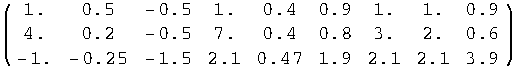
\includegraphics{refHmat.pdf}}}\intertext{with}
\psi_\epsilon=0, \,\,  \psi_z=I
\end{gather}
(\footnote{{refHmat.pdf}})
These coefficients  happen to produce a unique stable solution.
\begin{gather}
  B=
\vcenter{\hbox{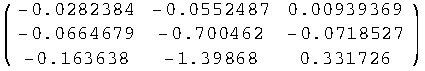
\includegraphics{refBmat.pdf}}}
\phi=
\vcenter{\hbox{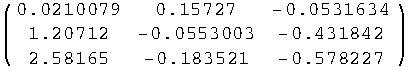
\includegraphics{refPhimat.pdf}}}\\
F=
\vcenter{\hbox{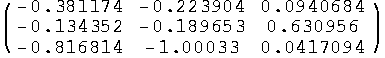
\includegraphics{refFmat.pdf}}}
\end{gather} (\footnote{files generated by demoApprox.mth}\footnote{{refBmat.pdf}})(\footnote{{refPhimat.pdf}})(\footnote{{refFmat.pdf}})
We can use the family of conditional expectations
along with the contrived reference model to recover an 
approximation for equation \refeq{soln} along with error bounds.
\footnote{Note that the reference model is deterministic and the $z$ functions account for the stochastic nature of the model.}
% \footnote{
% We need not  make these adjustments for the steady state,
% but doing so economizes on the number of terms 
% required for a given level of approximation
% accuracy.}

Using the following parameter values

\begin{gather}
\vcenter{\hbox{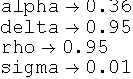
\includegraphics{RBCParamSubs.pdf}}} \,\, \text{ with } \,\,
  \begin{bmatrix}
    c_{ss}\\k_{ss} \\ \theta_{ss} \label{rbcparams}
  \end{bmatrix}=
\vcenter{\hbox{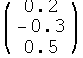
\includegraphics{RBCSSVal.pdf}}}
\end{gather}(\footnote{{RBCParamSubs.pdf}})(\footnote{{RBCSSVal.pdf}})

Should use ``stochastic steady  state''

\begin{gather}
 (\theta^\rho)e^{\frac{\sigma^2}{2}}=\theta > 1
\end{gather}

The contrived model can produce accurate values for the solution, but can require quite a few terms in the series to achieve a given level of accuracy. 
 Alternatively, as one might expect, developing 
a series using the model linearized about the ergodic mean produces a given
level of accuracy with 
fewer series terms.  

Note that the error bounds are useful in predicting how many terms are required for a given level of accuracy. Even the contrived model with randomly chosen
coefficients can achieve machine precision accuracy if one uses enough
terms from the series.  It also shows that adding new terms at some point becomes useless as rounding error limits any further improvement in the calculation.
This provides us some assurance that our iterative algorithm can be robust 
against errors if we include enough terms.

The table presents conservative estimates of the number of terms required
since the calculation uses the infinity norm.\footnote{Perhaps graph better.  Machine precision in tables.}  I estimate the infinity
norm by using a global maximization method to compute the largest value
attained by the infinity norm of the equation errors.\footnote{Why infinity norm?}  Column  blah shows that --- 

We can develop a robust algorithm since we can compute how many terms
we must compute in order to guarantee a particular level of accuracy.
I computed the largest infinity norm for the product of h over a range of
reasonable values.  

Algorithm will allow us to construct approximation along with error bounds on the resulting approximations.\footnote{file generated by demoApprox.mth -- {./rbcApprox.csv,./notRbcApprox.csv}}


We typically do not have exact solutions for the models of interest.
We can use these formulas to construct error bounds for solutions obtained by 
whatever method other methods.
Just pick a linear reference model.  Compute a bound on the discrepancy 
generated by substituting in the model constraints. between the model computed solutions and the 

%if problems with pgfplots, could be problem with auto include .cab files
%texpad people say force include
% use comment line like the following

%force-texpad-dependency:  file.ext

%see https://www.texpadapp.com/support/ios/file-management/non-standard-includes

 \begin{table}
   \centering
    
% \pgfplotstabletypeset[col sep=comma,
% columns/0/.style={column type=|c,int detect,column name=N},
% columns/1/.style={column type=|c,column name=Max Z},
% columns/2/.style={column type=|c,column name=Trunc Error Matrix},
% columns/3/.style={column type=|c,column name=Bound},
% columns/4/.style={column type=|c|,column name=Actual},
% every head row/.style={before row={\hline \multicolumn{5}{|c|}{``Arbitrary'' Linear Model}\\ \hline}},
% every last row/.style={after row={\hline }}
% ]{./notRbcApprox.csv}

\framebox{Table will show truncation errors for the ``Arbitrary'' Linear Model}

   \caption{Truncation Errors: Bound and Actual}
 \label{truncTab}
 \end{table}



 \begin{table}
   \centering

% \pgfplotstabletypeset[col sep=comma,
% columns/0/.style={column type=|c,int detect,column name=N},
% columns/1/.style={column type=|c,column name=Max Z},
% columns/2/.style={column type=|c,column name=Trunc Error Matrix},
% columns/3/.style={column type=|c,column name=Bound},
% columns/4/.style={column type=|c|,column name=Actual},
% every head row/.style={before row={\hline \multicolumn{5}{|c|}{Linearized RBC Model}\\ \hline }},
% every last row/.style={after row={\hline }}
% ]{./rbcApprox.csv}

\framebox{Table will show truncation errors for the  Linearized RBC Model}


   \caption{Truncation Errors: Bound and Actual}

 \end{table}



\section{Discovering Unknown Solutions}
\label{sec:unknown-solutions}

This section will require a lot more work!!!!

This section will describe how given the auxiliary ``chuck'' variables
and the linearity of the $Z$ functions in the series representation
that conditional expectations are straightforward to compute at each stage.
That is, we begin assuming the conditional expectations are given by the
linear reference model.  The solution at time $t$ is deterministic.
Provided we can solve it, we have determined the deterministic $z$ functions
that depend on $x_{t-1}$ and $\epsilon_t$.  For the next iteration,
we can use the given the distribution of $\epsilon$
we can compute the expected value
of these functions conditional on a given $x_t$.  This is again a deterministic
problem, admittedly with the complication that changes
$x_t$ moves the entire future, but we have a formula and a family of conditional
$Z$ functions to accommodate this fact. 


For unknown solutions we will need a way to generate the decision rule.  
Our initial strategy will be to solve 
relax the requirement for a time invariant solution and to solve
the model for a single period, then two, then three etc. We will monitor the
quality of the decision rule as described above and terminate when we 
can guarantee that the lotion satisfies a bound close to the exact solution.
Can describe this algorithm without approximations as follows:


Approximations are linear functions of the errors.  Just weighted by Z's.
Given an approximation from one function can just add the difference between the two  to get a new function approximation.



There are typically many solutions that satisfy the model equations and associated constraints.  For example, one could vary the probability distribution for $\epsilon_t$ or use perfect foresight to obtain a variety of solutions that
satisfy the model equations over time. But, for a given choice of probability distribution one may find there is a unique, at least locally, set of trajectories.


\begin{itemize}
\item $\mathcal{Z}^k(x) \implies (\xNow{k+1},\zNow{k+1}) \implies \mathcal{Z}^{k+1}(x)$  only the fixed point xguess for each value of $x_{t-1},\epsilon_t$ matters -- remember (memoize?)
\end{itemize}



Define $\XZPair{0}\equiv(B x_{t-1}+ \phi \psi_\epsilon\epsilon_{t} +
 (I - F)^{-1} \phi \psi_c,0)$.

Now, given
\begin{gather}
  \{\XZPair{0},\ldots,\XZPair{k}\}\intertext{ find }
\zNow{k+1} \ni \xNow{k+1} \intertext{satisfies Equation \refeq{theProblem} where}
  \xNow{k+1}\equiv B x_{t-1} + \phi \psi_\epsilon \epsilon_t + (I - F)^{-1} \phi \psi_c +  \phi \zNow{k+1}+
  \begin{cases}
0& \mbox{if }k=0\\    
\sum_{s=1}^{k} F^s \phi  \mathcal{Z}^{k+1-s}(x_{t+s}^k)&\mbox{if } k>0
  \end{cases}
\\
  x_{t+s}^{k+1}=\xIter{p}{ x_{t+s-1}^{k+1}}
  \begin{cases}
p=k+1-s &1\le s\le k+1\\
p=0 &s> k+1
  \end{cases}\intertext{to construct}
\ZNow{k+1}{}{}\equiv\mathcal{H}^{PF}[\zNow{k+1}] \text{ and }
\XNow{k+1}{}{}\equiv\mathcal{H}^{PF}[\xNow{k+1}] 
\intertext{ or }
\ZNow{k+1}{}{}\equiv\mathcal{H}^{RE}[\zNow{k+1}]\text{ and }
\XNow{k+1}{}{}\equiv\mathcal{H}^{RE}[\xNow{k+1}]
\end{gather}

At time t iteration $k+1$ we solve the system
\begin{gather}
 h(x_{t-1},\xNow{k+1}\xNowtp{k+1},\epsilon_{t})=0\\
% m(x_{t-1},\xNow{k+1}\xNowtp{k+1},\epsilon_{t}) \ge 0\\
   \end{gather}
If the problem arises from some optimization problem, 
it may prove useful to consider the associated Lagrangian.  In that case the $m$ equations and the Lagrange multiplies would be absorbed into the set of $h$ and $m$ need not explicitly appear.



By construction for $k\ge 0$
\begin{gather}
h(x_{t-1},g^{k+1}(x_{t-1},\epsilon_{t}),\mathcal{H}[g^{k+1}(g^{k+1}(x_{t-1},\epsilon_{t}),\epsilon_{t+1})],\epsilon_{t})=0 \intertext{ and for $ 1\le s\le k$}
\mathcal{H}[h(x_{t+s-1}^{k+1}(x_{t-1},\epsilon_t),x_{t+s}^{k+1}(x_{t-1},\epsilon_t),x_{t+s+1}^{k+1}(x_{t-1},\epsilon_t),\epsilon_{t+s})]=0 \intertext{we compute}
\discr{k+1}\equiv \mathcal{H}[h(x_{t+k}^{k+1}(x_{t-1},\epsilon_t),x_{t+k+1}^{k+1}(x_{t-1},\epsilon_t),x_{t+k+2}^{k+1}(x_{t-1},\epsilon_t),\epsilon_{t+k+1})]
\end{gather}
We use $\discr{k+1}$ as a measure of the potential impact of 
computing the remaining terms in the 
series expansion.  Under certain conditions, we can use this measure to compute and upper bound on the accuracy of the series function approximation.

Compute solution for $Z_k$ for path of length k.  For fixed point, path errs should be zero through k, with error at k+1 if Z was not approximated. 
Iteration without approximation leads to many many function evaluations as each successive Z calculation entails a fixed point calculation for the xz pairs.

Will have to approximate  $Z$  could use projection or interpolation or something else?  can use information from the stage of solution to decide on degree of approximation.  start of in accurate, add accuracy as get close.  different strategies for different problems.  More evaluations where function changes more.  
Bound infinity norm or other criteria.  could randomize points do approx alternatives in parallel.  assess the utility of any given and then proceed.

Even bad approximations iterated settle down to some particular value depending on the relationship between the reference model and the actual model.  If they have the same long run conditional expectations the ref model approximation errors will improve over over iteration period

reusing the latest will likely improve the path errs. getting a fixed point may not be worth it. especially if not doing approximation

Having computed the $z$ and $Z$ funcs for a given truncation horizon, T, we could compute the path which solves the system exactly for those T periods, but this will differ from the true solution.  We can bound the difference by checking the error at T+1.  

If the path error is zero or small enough, the z functions won't change.  We could possibly accelerate the process by using recently updated Z funcs further along the path in determining the path.  This should result in a decision rule that more closely approximates the true decision rule but requiring a shorter path to compute.

Provide a couple of iterations and monitor the number of function evaluations
the number of evaluations for fixed point for perfect foresight and for
rational expectations.  The computational costs quickly become prohibitive.

We can solve small models without any approximations for short horizons, but


\subsection{Exact Symbolic Solutions?}
\label{sec:exact-symb-solut}
If function compositions remain simple possible to solve exactly.


There are some short cuts as in precomputing the Z, so that at each step there are fewer calculations to make.  

But ultimately we will  need to make approximations.



\subsection{Constructing an Approximation: Problem Restatement}
\label{sec:constr-an-appr}



We will be interested in finding solutions for models that can be written in  the form


\begin{gather}
  h_i(x_{t-1},x_{t},x_{t+1},\epsilon_t)=h^{det}_{io}(x_{t-1},x_{t},\epsilon_t)+\sum_{j=1}^{p_i} [h^{det}_{ij}(x_{t-1},x_{t},\epsilon_t)h^{nondet}_{ij}(x_{t+1})]=0
\end{gather}
This is a very broad class of models and most economic models can 
be cast in this form.  

For example, the Euler equations for the  neoclassical growth  model 
\label{sec:simple-rbc-model-ext} can be written as
\begin{gather}
h_{10^{det}}(\cdot)=\frac{1}{c_t},\,\,
h_{11}^{det}()=\alpha \delta k_{t}^{\alpha-1} ,\,\,
h_{11}^{nondet}(\cdot)=E_t \left (\frac{\theta_{t+1}}{c_{t+1}} \right )\\
h_{20}^{det}(\cdot)=c_t + k_t-\theta_tk_{t-1}^\alpha,\,\,
h_{21}^{det}(\cdot)=0\\
h_{30}^{det}(\cdot)=\ln \theta_t -(\rho \ln \theta_{t-1} + \epsilon_t),\,\,
h_{31}^{det}(\cdot)=0
\end{gather}
Since we will be working with models where expectations are computed at time t, $\epsilon_t$ is known and the only stochastic components are those with time subscripts greater than $t$. We will need to compute 
the conditional expectation of nonlinear expressions,  
this specification will allow us to include auxiliary
variables that we will include in the augmented model for 
accurately recursively computing  the appropriate expected values.
Below, we will consider 
systems that augment these dynamic equations with additional constraints 
on the evolution of the variables.


We will be interested in
finding a time invariant function $g^\ast$ that satisfies
\begin{gather}
  \begin{split}
h(x_{t+s-1},g^\ast(x_{t+s-1},\epsilon_{t+s}),\mathcal{H}[g^\ast(g^\ast(x_{t+s-1},\epsilon_{t+s}),\epsilon_{t+s+1})],\epsilon_{t+s}) \label{theProblem} \\
%m(x_{t+s-1},g^\ast(x_{t+s-1},\epsilon_{t+s}),\mathcal{H}[g^\ast(g^\ast(x_{t+s-1},\epsilon_{t+s}),\epsilon_{t+s+1})],\epsilon_{t+s}) \ge 0  
  \end{split}
%  \intertext{define} 
% \mathcal{G}^\ast(x_{t+s-1},\epsilon_{t+s})= \mathcal{H}[g^\ast(g^\ast(x_{t+s-1},\epsilon_{t+s}),\epsilon_{t+s+1})] \nonumber
 \end{gather}
 for all $s>0$ where $\mathcal{H}$ is an operator, 
  that maps stochastic functions of $x$ and $\epsilon$ into deterministic 
functions of $x$ alone.  In this paper we will consider two such operators:



Could be any function that ``integrates out'' the $\epsilon$ so long as 
iterated ``expectations'' enforced.


\begin{description}
\item[Perfect Foresight]
\begin{gather}
     \mathcal{H}^{PF}[g^{k}(x,\epsilon_{t+T-k+1})]=
g^{k}(x,0)\\
\end{gather}


\item[Rational Expectations] 
\begin{gather}
     \mathcal{H}^{RE}[g^{k}(x,\epsilon_{t+T-k+1})]=
\mathcal{E}_t[g^{k}(x,\epsilon_{t+T-k+1})|x]\\
\end{gather}

 \end{description}












In what follows, we will use a representation like equation \refeq{theTruncSeries} 
to construct a sequence of functions, $g^k$, 
that will approximate the typically unknown solution $g^\ast$.
If we knew $g^\ast$, and  these function generate a bounded family of 
trajectories, we could define $z(x_{t+s-1},\epsilon_t)$ using \refeq{defZ}.
Constructing a companion linear model would subsequently allow 
 us to write down a series representation for the $g^\ast$ functions.  Below, we will show how to ``reverse engineer'' the series representation for $g^\ast$.






We begin by choosing some linear model of appropriate dimension that 
has a uniquely convergent steady state.  
Although this is not necessary, it may be possible to obtain this model by
linearizing the original model around the deterministic steady state.\footnote{As noted above, one could construct a series representation using any linear
 model of appropriate dimension with a unique stable solution.  The rate of convergence and the number of terms required for a  given level of accuracy will depend upon the linear model employed.}


 \begin{gather}
 g^0(x_{t-1},\epsilon_{t})=  
B x_{t-1}+ \phi \psi_\epsilon\epsilon_{t} +
 (I - F)^{-1} \phi \psi_c\\ \label{firstIter}
z^{0}_{t+i}(x_{t-1},\epsilon_{t-1})=0 \,\, \forall i \ge 0
 \end{gather}
We are now in a position to easily compute 
 \begin{gather}
\xIter{0}{x}=\mathcal{H}^{PF}[g^{0}(x,\epsilon_{t-k+1})]=
\mathcal{H}^{RE}[g^{0}(x,\epsilon_{t-k+1})]= 
B x+  (I - F)^{-1} \phi \psi_c
 \end{gather}
\begin{gather}
\underbrace{x_{t-1},0} 
\underbrace{\xNow{0},\zNow{0}}
\underbrace{\xNowtp{0}=\xIter{0}{x_{t}},0}
\end{gather}
In other words, from time t onwards, this approximation assumes 
that our stand-in
 convergent linear model completely characterizes the solution.\footnote{
The algorithm terminates with an approximation for 
the time invariant function $g^\ast$.}  It is unlikely that $g^0(x_{t-1},\epsilon_{t})$
satisfies equation \refeq{theProblem} for arbitrary $x_{t-1}$ even for $s=0$.
We can get a pessimistic upper bound for how far we are away from the solution 
by computing the infinity norm of substituting the variables from into Equation \refeq{theProblem}.\footnote{The values in Table \ref{truncTab} illustrate how
pessimistic this approximation can be, but it turns out we can expect the accuracy of  approximate truncation errors improve as we expand the approximation series.}

Next, we compute a solution in which the nonlinear equations are satisfied at time t alone while the stand-in linear system holds sway subsequently.
Our algorithm will  compute
\begin{gather}
\underbrace{x_{t-1},0} 
\underbrace{\xNow{1},\zNow{1}}
\underbrace{\xNowtp{1}=\xIter{1}{x_{t+1}},0}
\underbrace{\xNowtp{1}=\xIter{0}{x_{t+1}},0}
\end{gather}
that satisfy the nonlinear equation system at time t.
For a given $x_{t-1}$, we substitute
\begin{gather}
x_{t-1}, \,\,
  x_t=B x_{t-1} + \phi z^1(x_{t-1},\epsilon_t) , \,\,
  x_{t+1}=B x_{t} + \phi \mathcal{Z}^1(x_t)
\end{gather}
into the non linear equation system to determine the 
$z^1(x_{t-1},\epsilon_t)$ and consequently $x_t^1(x_{t-1},\epsilon_t)$.
We then have
 \begin{gather}
 g^1(x_{t-1},\epsilon_{t})=  
B x_{t-1}+ \phi \psi_\epsilon\epsilon_{t} +
\phi \psi_\epsilon z^1(x_{t-1},\epsilon_t)+
 (I - F)^{-1} \phi \psi_c\\ \label{firstIter}
z^{1}_{t+i}(x_{t-1},\epsilon_{t-1})=0 \,\, \forall i \ge 1
 \end{gather}
Now, $g^1(x_{t-1},\epsilon_{t})$
satisfies equation \refeq{theProblem} for arbitrary $x_{t-1}$ at time $t$ with $s=0$.  However, it probably does not solve the system for $s>0$.
We can get a pessimistic upper bound for how far we are away from the solution 
by substituting the variables and computing the infinity norm for plausible values of $x_{t-1}$.
\begin{gather}
\xNow{1},\xNowtp{1},\xNowtp{1}=\xIter{1}{x_{t+1}}
\end{gather}
into Equation \refeq{theProblem}. If the accuracy of the approximation is adequate, we need not compute any further  terms in the power series.  If not,
we are now in a position to compute our choice of
$\mathcal{Z}^1(x)=\mathcal{H}^{PF}[g^{1}(x,\epsilon_{t-k+1})]$ or
$\mathcal{Z}^1(x)=\mathcal{H}^{RE}[g^{1}(x,\epsilon_{t-k+1})]$.

%  \begin{gather}
%  g^0(x_{t-1},\epsilon_{t})=  
% B x_{t-1}+ \phi \psi_\epsilon\epsilon_{t} +
%  (I - F)^{-1} \phi \psi_c\\ \label{firstIter}
% z^{0}_{t+i}(x_{t-1},\epsilon_{t-1})=0 \,\, \forall i \ge 0
%  \end{gather}
%  \begin{gather}
%  g^0(x_{t-1},\epsilon_{t})=  
% B x_{t-1}+ \phi \psi_\epsilon\epsilon_{t} +
%  (I - F)^{-1} \phi \psi_c\\ \label{firstIter}
% z^{0}_{t+i}(x_{t-1},\epsilon_{t-1})=0 \,\, \forall i \ge 0
%  \end{gather}

Using these functions we can then compute a solution for a model whose trajectories satisfy equation system \refeq{rbcSys}
for two time periods and satisfy equation \refeq{rbcLinSys} subsequently.

\begin{gather}
\underbrace{x_{t-1},0}
\underbrace{\xNow{2},\zNow{2}} 
\underbrace{\xNowtp{2}=\XNow{2}{t}{t},\ZNow{2}{1}{t}}
\underbrace{\XNow{1}{t+1}{t},0}\underbrace{\XNow{0}{t+2}{t+1},0}    \intertext{where we have solved for $\xNow{2}$ and $\zNow{2}$ to satisfy the  equation system \refeq{theProblem}.}
\xNowtp{2}=\XNow{1}{t}{t}
\end{gather}

\begin{gather}
  \label{eq:1}
  x_t=B x_{t-1} + \phi z^2(x_{t-1},\epsilon) + F \phi \mathcal{Z}^1(x_t)\\
  x_{t+1}=B x_{t} + \phi \mathcal{Z}^1(x_t)+
 (I - F)^{-1} \phi \psi_c\\
  x_{t+2}=B x_{t+1} + (I - F)^{-1} \phi \psi_c\\
  x_{t+3}=B x_{t+2} + (I - F)^{-1} \phi \psi_c
\end{gather}

The next iteration highlights an aspect of the algorithmic step which allows us
to continue to exploit the law of iterated expectations in discovering the
solution for the model.
{\small
\begin{gather}
\underbrace{x_{t-1},0}
\underbrace{\xNow{3},\zNow{3}} 
\underbrace{\xNowtp{3}=\XNow{3}{t}{t},\ZNow{3}{1}{t}} 
\underbrace{\XNow{2}{t+1}{t},\ZNow{2}{2}{t+1}} 
\underbrace{\XNow{1}{t+3}{t+2},0}
\underbrace{\XNow{0}{t+4}{t+3},0}
\end{gather}
}

\begin{gather}
  \label{eq:1}
  x_t=B x_{t-1} + \phi z^3(x_{t-1},\epsilon) + F \phi \mathcal{Z}^2(x_t)+ F^2 \phi \mathcal{Z}^1(x_t)+
 (I - F)^{-1} \phi \psi_c\\
  x_{t+1}=B x_{t} + \phi \mathcal{Z}^1(x_t)+ F^2 \phi \mathcal{Z}^1(x_t)+
 (I - F)^{-1} \phi \psi_c\\
  x_{t+2}=B x_{t+1} + (I - F)^{-1} \phi \psi_c\\
  x_{t+3}=B x_{t+2} + (I - F)^{-1} \phi \psi_c\\
  x_{t+4}=B x_{t+2} + (I - F)^{-1} \phi \psi_c
\end{gather}



In the general iteration step we will have
\begin{gather}
  \label{eq:1}
  x_t=B x_{t-1}  \phi \psi_\epsilon \epsilon_t + (I - F)^{-1} \phi \psi_c +
\sum_{s=0}^{k} F^s \phi \mathcal{Z}^{k-s}(x_{t+s}^{k+1})\\
  x_{t+s}^{k+1}=\Pi_{s=0}^k \xIter{s}{ x_{t}^{k+1}}
\end{gather}




\begin{description}
\item[operation counts] 
\item[Time] 
\item[Space] 
\end{description}

\subsubsection{Function Approximation}
\label{sec:funct-appr}

\begin{itemize}
\item for perfect foresight easier and faster than for rational expectations 
\end{itemize}

We will first focus on approximating the functions by abstracting for the expectations calculation and sorting out perfect foresight solutions.
\paragraph{Projection}



\paragraph{Interpolation}

\paragraph{Smolyak}

\subsubsection{Expectations Integral Approximation}
\label{sec:funct-appr}

Note that $\XtFuncTI$  requires integrating linear functions of the $Z$.


It may not be necessary to compute expectations accurately at the initial stages of the algorithm.  These become future values whose errors will be discounted by the F matrix multiplications.  Once in the vicinity of the solution
tightening up the Z calculation could accelerate convergence.


One could consider Tauchen approach for expectations.  Not particularly high
dimensional integration since just one period at a time.


\subsection{A Simple RBC Model Example}
\label{sec:simple-rbc-model-1}


In most ways, this is a good example because there is a closed form solution
and the model is well known and widely used as a foundation for other DSGE
models.  It has the unfortunate aspect that perfect foresight solution 
coincides with the rational expectations solution.  As a result it will be
useful to consider the model with CRRA but not Log utility.\footnote{Iterating on the whole path, one likely will encounter basins of attraction between solutions.  For example starting near a perfect foresight solution, may drive one to the perfect foresight solution.  Starting close to a particular rational expectations solution might leave one there.  For the RBC model in the text, the distribution}


\subsubsection{Recovering the Known Solution:  $U(c) = Log(c)$}
\label{sec:recov-known-solut}




\paragraph{For T=1 Machine Precision}
\label{sec:t=1}

Show simplicity and how this will help solve difficult problems.  
This core computation gets repeated the most so should be efficient. Has big
impact on tractability after break link for iteration step using approximation.


We will need to solve a nonlinear equation system to obtain the values of $z$ for a given set of initial conditions.  For this problem the problem is 
deterministic and can be rather difficult. 
The problem can be nonlinear, it can
have inequality constraints, it can have regime changes.  So long as we can
compute a solution and then apply our ``expectations operator'' we can 
proceed to the next step.

\begin{itemize}
\item examples
\item function evaluations
\item time
\item accuracy
\end{itemize}



\paragraph{For T=2  Machine Precision}
\label{sec:t=1}

Show modest compromise  of 
simplicity and how this will help solve difficult problems.  
This core computation gets repeated the most so should be efficient. Has big
impact on tact-ability after break link for iteration step using approximation.


For T=2 the future $z$ depends on $x$ which depends on the current $z$.
We need to solve these simultaneously. 
It appears that simple iteration seems to work fine to provide a fixed point.  


\begin{itemize}
\item examples
\item function evaluations
\item time
\item accuracy
\end{itemize}



\paragraph{For T=3  Machine Precision}
\label{sec:t=1}


Show modest compromise  of 
simplicity and how this will help solve difficult problems.  
This core computation gets repeated the most so should be efficient. Has big
impact on tractability after break link for iteration step using approximation.

But Show increase in findroots.

Possible but costly.
For T=3 the future $z$ depends on $x$ which depends on the current $z$.
We need to solve these simultaneously. 
It appears that simple iteration seems to work fine to provide a fixed point.  

Show increase in findroots.


\begin{itemize}
\item examples
\item function evaluations
\item time
\item accuracy
\end{itemize}

\begin{itemize}
\item Stick t solving path or
\item loop on fixed point for Z
\item accuracy and costs
\end{itemize}



Needs generalization of ``chunk'' $\frac{1}{c_t}\rightarrow \left (\frac{\theta_{t+1}}{c_{t+1}^\eta} \right )$

We construct our stand-in model by augmenting the model with the equation
\begin{gather}
  \rcpC_t=\frac{1}{c_t}
\end{gather}
substituting $\rcpC_{t+1}$ for $\frac{1}{c_{t+1}}$ in the first equation and 
 linearizing the RBC model about the ergodic mean
given in \refeq{rbcparams}
\begin{gather}
  \begin{bmatrix}
H_{-1}&H_{0}&H_{1} 
  \end{bmatrix}=
\vcenter{\hbox{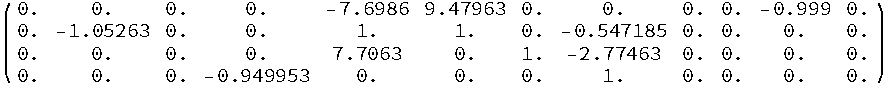
\includegraphics{RBCHmatSymb.pdf}}} \label{rbcLinSys}
\intertext{with}
\psi_\epsilon=
\begin{bmatrix}
  0\\0\\1\\0
\end{bmatrix}, \psi_z=I
\end{gather}(\footnote{generated by AMAPaperCalcs.mth {RBCHmatSymb.pdf}})

These coefficients  produce a unique stable linear solution.

\begin{gather}
  B=
\vcenter{\hbox{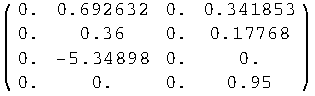
\includegraphics{RBCBmatSymb.pdf}}},
\phi=
\vcenter{\hbox{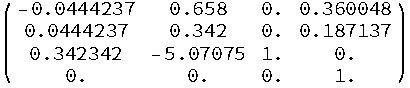
\includegraphics{RBCPhimatSymb.pdf}}}\\
F=
\vcenter{\hbox{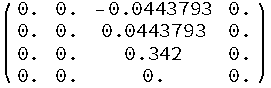
\includegraphics{RBCFmatSymb.pdf}}}\\
\psi_c=
\vcenter{\hbox{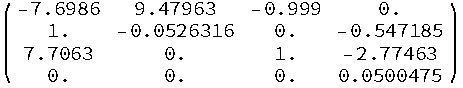
\includegraphics{RBCHSum.pdf}}}
\vcenter{\hbox{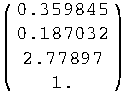
\includegraphics{RBCSS.pdf}}}=\vcenter{\hbox{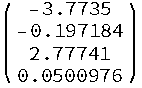
\includegraphics{RBCPsissSymb.pdf}}}
\end{gather}(\footnote{generated by AMAPaperCalcs.mth {RBCBmatSymb.pdf}})(\footnote{generated by AMAPaperCalcs.mth {RBCPhimatSymb.pdf}})(\footnote{generated by AMAPaperCalcs.mth {RBCFmatSymb.pdf}})(\footnote{generated by AMAPaperCalcs.mth {RBCHSum.pdf}})(\footnote{generated by AMAPaperCalcs.mth {RBCSS.pdf}})

Applying the formula \refeq{firstIter} produces:

{\tiny
\begin{gather}
  \begin{bmatrix}
c_t\\k_t\\ \rcpC_t\\\theta_t
  \end{bmatrix}=%paperCalcsRBCExample xt00
   \left(
   \begin{array}{c}
 0.359845 \epsilon _t+0.692632 k_{t-1}+0.341853 \theta _{t-1}-0.0442851
   \text{z1}_{t-1}+0.658 \text{z2}_{t-1}+0.359845 \text{z3}_{t-1}-0.111552 \\
 0.187032 \epsilon _t+0.36 k_{t-1}+0.17768 \theta _{t-1}+0.0442851
   \text{z1}_{t-1}+0.342 \text{z2}_{t-1}+0.187032 \text{z3}_{t-1}-0.0579799 \\
 -5.34898 k_{t-1}+0.342 \text{z1}_{t-1}-5.08153
   \text{z2}_{t-1}+\text{z4}_{t-1}+3.7794 \\
 \epsilon _t+0.95 \theta _{t-1}+\text{z3}_{t-1}+0.05 \\
   \end{array}
   \right)
\end{gather}
}

and 


{\tiny
%xt01=Private`computeNextXt[{Private`bmat,Private`phimat,Private`fmat,Private`psieps,Private`psic,Private`psiz},solnFunc00PF[[3+Range[3]]],{{cc},{kk},{tt}},{1}]//N//Expand//Simplify
\begin{gather}
  \begin{bmatrix}
c_{t+1}\\k_{t+1}\\ \rcpC_{t+1}\\\theta_{t+1}
  \end{bmatrix}=%paperCalcsRBCExample xt00
  \left(
   \begin{array}{c}
 0.471397 \epsilon _t+0.249347 k_{t-1}+0.447827 \theta _{t-1}+0.0306732
   \text{z1}_{t-1}+0.23688 \text{z2}_{t-1}+0.471397 \text{z3}_{t-1}-0.134618 \\
 0.245012 \epsilon_t+0.1296 k_{t-1}+0.232761 \theta _{t-1}+0.0159426
   \text{z1}_{t-1}+0.12312 \text{z2}_{t-1}+0.245012 \text{z3}_{t-1}-0.0699687 \\
 -1.00043 \epsilon _t-1.92563 k_{t-1}-0.950409 \theta _{t-1}-0.23688
   \text{z1}_{t-1}-1.82935 \text{z2}_{t-1}-1.00043 \text{z3}_{t-1}+4.08954 \\
 0.95 \epsilon _t+0.9025 \theta _{t-1}+0.95 \text{z3}_{t-1}+0.0975 \\
   \end{array}
   \right)
\end{gather}}

Substituting  these expressions into equation \refeq{rbcSys} produces
a deterministic system such that, given specific values for 
$(x_{t-1},\epsilon_{t})=(c_{t-1}, k_{t-1},\rcpC_{t-1}, \theta_{t-1}, \epsilon_t)$, we can solve for $z_{1t}(x_{t-1},\epsilon_{t})$, $z_{2t}(x_{t-1},\epsilon_{t})$, $z_{2t}(x_{t-1},\epsilon_{t})$, and $z_{4t}(x_{t-1},\epsilon_{t})$  completely determining
$c_{t}(x_{t-1},\epsilon_{t})$, $k_{t}(x_{t-1},\epsilon_{t})$, $\rcpC_{t}(x_{t-1},\epsilon_{t})$  and $\theta_{t}(x_{t-1},\epsilon_{t})$.\footnote{In this example, the lagged value,  $c_{t-1}$ does not appear in the equation system and consequently plays no role in determining the solution.}  In effect we have 
computed a solution for a model whose trajectories satisfy equation system \refeq{rbcSys}
for one time period and satisfy equation \refeq{rbcLinSys} subsequently. As can
be seen in the top panel of Figure \ref{fig:cfuncfirst}, 
imposing the constraint for even a single period captures much of the non linearity, but the bottom panel shows that the solution is 
still significantly far away from the exact solution.


Number of function evaluations and time.

fixed point not necessary.

find root must use genxz func
takes time to construct function for findroot  called twice by fixed point, but solution guaranteed on second call.

%\includegraphics[height=8.0in]{conExpPathsNote.pdf}(\footnote{{conExpPathsNote.pdf}})



Took 0.01 seconds while profiling.  Findroot called the xz func about 30 times.
\begin{figure}
  \centering
%\includegraphics{cFuncExt00Lin.pdf}(\footnote{{cFunc00Lin.pdf}})
  \caption{Solution for c imposing non linear model constraints for a single period}
%\includegraphics{cFuncExt00Exact.pdf}(\footnote{{cFunc00Exact.pdf}})
  \caption{Solution for c imposing non linear model constraints for a single period}
  \label{fig:cfuncfirst}
\end{figure}

We are now in a position to compute
$\mathcal{H}^{PF}[g^{0}(x,\epsilon_{t-k+1})]$ or
$\mathcal{H}^{RE}[g^{0}(x,\epsilon_{t-k+1})]$.
Using these functions we can then compute a solution for a model whose trajectories satisfy equation system \refeq{rbcSys}
for two time periods and satisfy equation \refeq{rbcLinSys} subsequently.
\begin{gather}
  \label{eq:1}
  x_t=B x_{t-1} + \phi z_0(x_{t-1},\epsilon) + F \phi \mathcal{Z}^1(x_t)\\
  x_{t+1}=B x_{t} + \phi \mathcal{Z}^1(x_t)
\end{gather}
{\tiny

\begin{gather}%paperCalcsRBCExample.mth xt01
  \label{eq:2}
   \left(
   \begin{array}{c}
 0.359845 \epsilon _t+0.692632 k_{t-1}+0.341853 \theta _{t-1}-0.0442851
   \text{z1}_{t-1}-0.0442851 \text{Z1}_{t-1}+0.658 \text{z2}_{t-1}+0.359845
   \text{z3}_{t-1}+0.225036 \text{Z3}_{t-1}-0.0151455 \text{Z4}_{t-1}-0.111552 \\
 0.187032 \epsilon _t+0.36 k_{t-1}+0.17768 \theta _{t-1}+0.0442851
   \text{z1}_{t-1}+0.0442851 \text{Z1}_{t-1}+0.342 \text{z2}_{t-1}+0.187032
   \text{z3}_{t-1}-0.225036 \text{Z3}_{t-1}+0.0151455 \text{Z4}_{t-1}-0.0579799 \\
 -5.34898 k_{t-1}+0.342 \text{z1}_{t-1}+0.342 \text{Z1}_{t-1}-5.08153
   \text{z2}_{t-1}-1.73788 \text{Z3}_{t-1}+\text{z4}_{t-1}+0.116964
   \text{Z4}_{t-1}+3.7794 \\
 \epsilon _t+0.95 \theta _{t-1}+\text{z3}_{t-1}+0.05 \\
   \end{array}
   \right)
\end{gather}
}

{\tiny
  \begin{gather}
    \label{eq:3}
       \left(
   \begin{array}{c}
 0.471397 \epsilon _t+0.249347 k_{t-1}+0.447827 \theta _{t-1}+0.0306732
   \text{z1}_{t-1}-0.0578969 \text{Z1}_{t-1}+0.23688 \text{z2}_{t-1}+0.658
   \text{Z2}_{t-1}+0.471397 \text{z3}_{t-1}+0.429014 \text{Z3}_{t-1}-0.00465525
   \text{Z4}_{t-1}-0.134618 \\
 0.245012 \epsilon _t+0.1296 k_{t-1}+0.232761 \theta _{t-1}+0.0159426
   \text{z1}_{t-1}+0.104513 \text{Z1}_{t-1}+0.12312 \text{z2}_{t-1}+0.342
   \text{Z2}_{t-1}+0.245012 \text{z3}_{t-1}-0.119017 \text{Z3}_{t-1}+0.0205979
   \text{Z4}_{t-1}-0.0699687 \\
 -1.00043 \epsilon _t-1.92563 k_{t-1}-0.950409 \theta _{t-1}-0.23688
   \text{z1}_{t-1}+0.44712 \text{Z1}_{t-1}-1.82935 \text{z2}_{t-1}-5.08153
   \text{Z2}_{t-1}-1.00043 \text{z3}_{t-1}-0.534171 \text{Z3}_{t-1}+1.03595
   \text{Z4}_{t-1}+4.08954 \\
 0.95 \epsilon _t+0.9025 \theta _{t-1}+0.95 \text{z3}_{t-1}+\text{Z3}_{t-1}+0.0975 \\
   \end{array}
   \right)
  \end{gather}
}





\begin{figure}
  \centering
%\includegraphics{cFuncTwoPerErr.pdf}(\footnote{{cFuncTwoPerErr.pdf}})
 \caption{Solution for c imposing non linear model constraints for two periods}
%\includegraphics{cFuncThreePerErr.pdf}(\footnote{{cFuncThreePerErr.pdf}})
  \caption{Solution for c imposing non linear model constraints for three periods}
  \label{fig:cfuncsecond}
\end{figure}

\subsubsection{Approximating an Unknown Solution: $U(c) \ne Log(c)$ }
\label{sec:recov-known-solut}



\subsubsection{Occasionally Binding Constraints}
\label{sec:recov-known-solut}


\subsubsection{A Regime Switching Version}
\label{sec:regime-switch-model}



\cite{foerster13}

\begin{gather}
c_t + z_t k_t = z_t^{1-\alpha} k_{t-1}^\alpha + (1-\delta)k_{t-1}\\
 \log z_t = (1-\rho(s_t))\mu(s_t) + \rho(s_t)\log z_{t-1}+ \sigma(s_t) \epsilon_t\\
 c_t^{\gamma-1} = \beta  
 E_t ( c_{t+1}^{\gamma-1} (\alpha z_{t+1}^{1-\alpha} k_t^{\alpha -1} + (1-\delta) ))
\end{gather}


\section{Other Examples}
\label{sec:examples}

\anEdit{models should be well known.  Avoid spending time explaining a model.
Luca's JME paper 3rd model.\cite{Guerrieri2015}}

\anEdit{Explore what others have said about error bounds.  }



\subsection{The Burnside Model: a Model With Known Solution}

Another model with an exact solution can be found in \cite{burnside}
\begin{gather}
\normalsize y_t - \beta E_t \{ (1+y_{t+1}) exp{(\theta \bar{x} + \theta \sigma \epsilon_{t+1})} \} = 0\intertext{so that}
\end{gather}



\subsection{A Simple Financial Model: Occasionally Binding Constraints}
\label{sec:simple-financ-model}


Since the equations are linear, and only one of the equations has to change 
when the constraint binds, we only need to solve for one $z$:  the others 
are all zero.

\subsection{Precomputing Z Components}

Can reduce costs, but not fast enough relative to required findroots.

\begin{itemize}
\item backward looking nonlinear equations know values for the  $z$.  Even if depend on variables that aren't lagged the z discrepancy could be precomputed.
\item for known z, can precompute and determine how many terms need to compute before ignoring the impact
\item One need only construct and solve a system large enough to determine the non zero $z$-function.
\item any linear equation required to remains satisfied will have an identically zero z
\item for non linear variables that are completely backward looking one can solve for the z functions for those equations 
ahead of time( as well as just substitute them out )
\end{itemize}
Completely backward and completely forward variables pre compute



A model specification consists of
\begin{description}
\item[Uniquely convergent linear rational expectations model] 
We will need the $B, \phi, F, \psi_\epsilon, \psi_c \text{ and }\psi_z$ matrices
\item[A function that computes the current set of constraint given a path and the current set of z functions] 
  \begin{gather}
    \mathcal{C}(x_{t-1},x_{t},x_{t+1},z(x_{t-1},\epsilon_t))
  \end{gather}
\end{description}

\subsection{Smets and Woeters: a Moderate Sized DSGE}


\section{Future Directions}
\label{sec:implementation}
\begin{description}
\item[Applications] \ 

  \begin{itemize}
\item add factors for nonlinear models
\item nonlinear model ad factors ed 
\item time varying coefficients possible
\item seasonal factors
  \end{itemize}
\item[Extensions] \ 

  \begin{itemize}
\item consider models with multiple convergent stochastic steady states ( regime switching?)
\item other ``expectations'' operators
\item Formula also works for multilag multi lead.  Applications
\item the ``expectations operator'' could be generalized
  \end{itemize}
\item[Implementation] \ 

  \begin{itemize}
\item meta algorithm design components  on the fly.  interpolation parameters for example/  even more goal possible, look t computational burden forecast solution strategy
\item vary order of interpolation(approximation) for different variables
\item multitude of updating strategies for Z paths, true to path or accelerate perhaps blend t ensure convergence
\item parallel/GPU
\item there could be alternative solutions along the way to computing the path that lead to dead ends and frustrate convergence -- even if only one unique time invariant solution.
\item improve simulation performance via z feedback
\item use function composition evaluation to determine refined grid. possible that the set of refinements produce a fixed point  ( probably gives especially accurate interpolation
  \end{itemize}
\item[Proofs] \ 

  \begin{itemize}
  \item what about complex z
  \item can precomputing z's speed up Luca Mateo algorithm
  \item unit roots in F how to handle/exploit
  \item choosing the linear model.  pushing down on F eigenvalues
  \item existence and uniqueness of solutions
\item what if model doesn't have a solution or has many
\item f eigenvalue assumptions proof
\item linear space for models
\item can get non linear model z's then add constraints and have difference in z's to characterize differences in models
\item the program is the proof possible with category theory here?
\item lots of choices about choosing grid points each z could have different interpolation order or even mix Chebyshev and interpolation
\item Interpolate before or after integration
  \end{itemize}
\end{description}









  






\appendix
\newpage

\section{To Do}
\label{sec:do}

\begin{itemize}
\item For the occasionally binding, there are some trajectories that reengage even
with perfect foresight.
\item plot at grid points instead of 3DPlots
\item op counts, time accuracy
\item precompute Z
\item interpolation
\item eval DR must use DR integral and chunks
\item automate locating chunks
\item patherr a distribution
\item concentric rings: solve in ``easy region'' with short paths, expand outward
\item parallelism for finding good reason communicate move processor toward that area
\item which is better to characterize discrepancy, simulation via decision rule or discrepancy between the ``computed exact'' solution path  do they coalesce
\item re-factor function arg lists
\item machine precision cutoff for tables and graph
\item pitch functional programming
\end{itemize}
\section{The algorithms}
\label{sec:algorithms}

\begin{pseudocode}{solnSubs}{[c_{t-1},k_{t-1},\frac{1}{c_t},\theta_{t-1},\epsilon_t]}
\RETURN{Rules}  
\end{pseudocode}


\begin{pseudocode}{solnFuncs}{[\{c_{t-1},k_{t-1},\frac{1}{c_t},\theta_{t-1},\epsilon_t\}]}
\RETURN{Matrix}  
\end{pseudocode}

 \begin{gather}
 Through[funcsInterp[k_{t-1},\theta_{t-1},\epsilon_t] \rightarrow
 \begin{bmatrix}
   x_t\\x_{t+1}\\z_t
 \end{bmatrix}
 \\
 Through[funcsInterpPF[k_{t-1},\theta_{t-1}]\rightarrow
 \begin{bmatrix}
   x_t\\x_{t+1}\\z_t
 \end{bmatrix}
\\
 Through[funcsInterpRE[k_{t-1},\theta_{t-1}]\rightarrow
 \begin{bmatrix}
   x_t\\x_{t+1}\\z_t
 \end{bmatrix}
\\
 Through[ZZks[k_{t-1},\theta_{t-1}]\rightarrow
 \begin{bmatrix}
z_t
 \end{bmatrix}
\\
 \end{gather}


% \section{Things To Do}
% \label{sec:things-do}

% \begin{itemize}
% \item guess should also use shock
% \item code to check model definition functions' validity
% \item flesh out constraints on function in code and add to text
% \item describe fixed point and init guess  need to take account of shock to get fixedpoint to converge
%\item Volterra Series and Impulse Response Functions
% \end{itemize}

\section{Truncation Error Bounds}
\label{truncForm}
{
\begin{gather}
\phi \psi_c=  \sum_{s=0}^\infty F^s \phi \psi_c  -   F \sum_{s=0}^\infty F^s \phi \psi_c \\
(I-F) \left (\sum_{s=0}^\infty F^s \phi \psi_c \right ) =\phi \psi_c\\
\sum_{s=0}^\infty F^s \phi \psi_c=(I - F)^{-1}\phi \psi_c\\
\sum_{s=0}^{k+1} F^s \phi \psi_c=F \sum_{s=0}^{k} F^s \phi \psi_c + \phi \psi_c\\
F^{k+1} \phi \psi_c +\sum_{s=0}^{k} F^s \phi \psi_c=F \sum_{s=0}^{k} F^s \phi \psi_c + \phi \psi_c\\
(I -F)\sum_{s=0}^{k} F^s\phi \psi_c  = (I- F^{k+1}) \phi \psi_c\\
\sum_{s=0}^{k} F^s \phi \psi_c = (I -F)^{-1}(I- F^{k+1}) \phi \psi_c\\
\sum_{s=k+1}^{\infty} F^s \phi \psi_c = (I -F)^{-1} F^{k+1}\phi \psi_c
\end{gather}
}

\section{Probably Not Needed}


 \begin{gather}
 g^0(x_{t+T-1},\epsilon_{t+T})=  
B x_{t+T-1}+ \phi \psi_\epsilon\epsilon_{t+T} +
 (I - F)^{-1} \phi \psi_c\\ \label{firstIter}
z^{T,0}_{t+T+i}(x_{t+T-1},\epsilon_{t+T-1})=0 \,\, \forall i \ge 0
 \end{gather}
In other words, this approximation assumes 
that our stand-in convergent linear model completely characterizes the solution.\footnote{
The algorithm terminates with an approximation for 
the time invariant function $g^\ast$. }

 Our algorithm will use  
 \begin{gather}
 g^{k}(x_{t+T-(k+1)},\epsilon_{t+T-k}) \intertext{ and}
 \{ z^{T-k,k}(x_{t+T-(k+1)},\epsilon_{t+T-k}),\ldots, z^{T,k}(x_{t+T-(k+1)},\epsilon_{t+T-k})\}
   \end{gather}
  to solve for 
 \begin{gather}
 g^{k+1}(x_{t+T-(k+2)},\epsilon_{t+T-(k+1)}) \intertext{ and}
 \{ z^{T-(k+1),k+1}(x_{t+T-(k+2)},\epsilon_{t+T-(k+1)}),\ldots, z^{T,k+1}(x_{t+T-(k+2)},\epsilon_{t+T-(k+1)})\}
   \end{gather}





First, note that after completing any given step $k$
we  are in a position to compute the deterministic functions 
$\mathcal{G}^k$ and $\{\mathcal{Z}^{T-k,k},\ldots,\mathcal{Z}^{T,k}\}$:
\begin{gather}
   \mathcal{G}^{k}(x)= \mathcal{H}[g^{k}(x,\epsilon_{t+T-k+1})]\\
   \mathcal{Z}^{T-k+i,k}(x)= \mathcal{H}[z^{T-k+i,k}(x,\epsilon_{t+T-k+1})] \,\, i=0,\ldots,k. 
\end{gather} 

The iteration step proceeds as follows:

\begin{enumerate}
\item Write
\begin{align*}
g^{k+1}(x_{t+T-(k+2)},\epsilon_{t+T-(k+1)})=&\\
&B x_{t-1}+ \phi \psi_\epsilon\epsilon_t + \\
&\sum_{s=0}^{k+1} F^s \phi z^{T-(k+1)+s,k+1}_{t+s}(x_{t+T-(k+2)},\epsilon_{t+T-(k+1)}) +\\
& (I - F)^{-1} \phi \psi_c
\end{align*}
\item economize on updating some of
the $z^{T-k+i,k+1}(x_{t+T-(k+2)},\epsilon_{t+T-(k+1)})$ by composing known
deterministic functions with the as yet undetermined $g^{k+1}$
\begin{gather}
z^{T-k+i,k+1}(x_{t+T-(k+2)},\epsilon_{t+T-(k+1)})= \mathcal{Z}^{T-k+i,k}(g^{k+1}(x_{t+T-(k+2)},\epsilon_{t+T-(k+1)}) \,\, \\i=0,\ldots,k  
\end{gather}
 and
\item  use the functions in \refeq{theProblem} to determine the new functions 
 $g^{k+1}$  and  $z^{T-(k+1),k+1}$ %(x_{t+T-(k+2)},\epsilon_{t+T-(k+1)})


\begin{gather}
 h(x_{t+T-(k+2)},g^{k+1}(x_{t+T-(k+2)},\epsilon_{t+T-(k+1)}), \mathcal{G}^{k}(g^{k+1}(x_{t+T-(k+2)},\epsilon_{t+T-(k+1)})),\epsilon_{t+T-(k+1)})\\ \label{iterSys}
%m(x_{t+T-(k+2)},g^{k+1}(x_{t+T-(k+2)},\epsilon_{t+T-(k+1)}),\mathcal{G}^{k}(g^{k+1}(x_{t+T-(k+2)},\epsilon_{t+T-(k+1)})),\epsilon_{t+T-(k+1)}) \ge 0\\ 
 g^{k+1}(x_{t+T-(k+2)},\epsilon_{t+T-(k+1)})= 
 B x_{t+T-(k+2)}+ \phi \psi_\epsilon\epsilon_{t+T-(k+1)} +\\
\sum_{i=1}^k F^i \phi \mathcal{Z}^{T-k+i,k}(g^{k+1}(x_{t+T-(k+2)},\epsilon_{t+T-(k+1)})) +\\
 \phi z^{(T-(k+1)),k+1}_{t+i+(k+1)}(x_{t+T-(k+2)},\epsilon_{t+T-(k+1)})\\
   \end{gather}
\end{enumerate}

These steps will likely take place point by point and will require an interpolation or projection method to characterize the functions.

To determine $g_0(x_{t-1},\epsilon_t)$ we set

\begin{gather}
	 g_{0}(x_{t-1},\epsilon_t) =B x_{t-1}+ \phi \psi_\epsilon\epsilon_t + (I - F)^{-1} \phi \psi_c + \phi z^{T,0}_{T}(x_{t-1},\epsilon_t)
\\
	 \mathcal{G}^0(x) =B x + (I - F)^{-1} \phi \psi_c \nonumber
\end{gather}

and use  equation \refeq{iterSys} to determine the unknown $z_T(x_{T-1},\epsilon_T)$

\begin{gather}
 h(x_{t+T-1},\mathbf{x}_T,\mathbf{x}_{T+1},\epsilon_{t+T})=0\\
% m(x_{t+T-1},\mathbf{x}_T,\mathbf{x}_{T+1},\epsilon_{t+T}) \ge 0\\
 \intertext{ where }
\mathbf{x}_t=B x_{T-1}+ \phi \psi_\epsilon\epsilon_t + (I - F)^{-1} \phi \psi_c+ \phi z^{T,0}_{T}(x_{T-1},\epsilon_t)\\
\mathbf{x}_{t+1}=B(B x_{T-1}+ \phi \psi_\epsilon\epsilon_t + (I - F)^{-1} \phi \psi_c + \phi z^{T,0}_{T}(x_{T-1},\epsilon_t)) + (I - F)^{-1} \phi \psi_c\\
   \end{gather}




\begin{gather}
  \{g_k(x_{t-1},\epsilon_t),\mathcal{Z}^k_0(x), \ldots, \mathcal{Z}^{k-1}_k(x) \} \rightarrow \\
  \{g^{k+1}(x_{t-1},\epsilon_t),\mathcal{Z}^{k+1}_0(x), \ldots, \mathcal{Z}^{k}_{k+1}(x) \}
\end{gather}

The code employs a simple fixed point iteration for any given $x_{t-1},\epsilon_t$.
We begin by setting $[\prescript{0}{}{x}(x_{t-1},\epsilon_t)]=g_k(x_{t-1},\epsilon_t)$. We 
solve for $[\prescript{l+1}{}{x}(x_{t-1},\epsilon_t)]$ and $[\prescript{l+1}{}{z}(x_{t-1},\epsilon_{t})]$ in 


\begin{gather}
\{ h, m, B, \phi, F, \psi_\epsilon, \psi_z \}  \rightarrow\\
 h(x_{t-1},[\prescript{l+1}{}{x}(x_{t-1},\epsilon_{t})], \mathcal{G}^{k}([\prescript{l}{}{x}(x_{t-1},\epsilon_{t})]),\epsilon_{t})\\
%m(x_{t-1},[\prescript{l+1}{}{x}(x_{t-1},\epsilon_{t})],\mathcal{G}^{k}([\prescript{l}{}{x}(x_{t-1},\epsilon_{t})]),\epsilon_{t}) \ge 0\\
 [\prescript{l+1}{}{x}(x_{t-1},\epsilon_{t})]= 
 B x_{t-1}+ \phi \psi_\epsilon\epsilon_{t} +\\
\sum_{i=1}^k F^i \phi \mathcal{Z}^{k}_i(\mathbf{x}) +\\
 \phi [\prescript{l+1}{}{z}(x_{t-1},\epsilon_{t})]\intertext{ where}
\mathbf{x}=[\prescript{l+1}{}{x}(x_{t-1},\epsilon_{t})]\text{ or } [\prescript{l}{}{x}(x_{t-1},\epsilon_{t})]
   \end{gather}


We terminate when 
\begin{gather}
    \twoNorm{  \begin{bmatrix}
\prescript{l+1}{}{x}(x_{t-1},\epsilon_{t})-
\prescript{l}{}{x}(x_{t-1},\epsilon_{t})\\
\prescript{l+1}{}{z}(x_{t-1},\epsilon_{t})-
\prescript{l}{}{z}(x_{t-1},\epsilon_{t})
  \end{bmatrix}} \le \epsilon_{fp} = 10^{-10} \intertext{ with }
\begin{bmatrix}
{\hat{x}}(x_{t-1},\epsilon_{t})\\
{\hat{z}}(x_{t-1},\epsilon_{t})
\end{bmatrix}=
\begin{bmatrix}
\prescript{l+1}{}{x}(x_{t-1},\epsilon_{t})\\
\prescript{l+1}{}{z}(x_{t-1},\epsilon_{t})
\end{bmatrix}
\end{gather}

We compute 
$  \hat{g}(x_{t-1},\epsilon_{t})$ by either projection or interpolation.



\newpage

\href{http://www.dynare.org/DynareShanghai2013/deterministic.pdf}{Occasionally binding constraints in neoclassical growth model}

 \bibliographystyle{plainnat}
 \bibliography{../../bibFiles/anderson,../../bibFiles/files}

\end{document}


